% X-StreamRAG — IOE413 mini project report (IEEE two-column conference format).
% Compile on Overleaf (pdfLaTeX) with the figures in report/figures/.
% Every number in Section VI comes from results/<run_id>/metrics.json.
\documentclass[conference]{IEEEtran}
\usepackage{graphicx}
\usepackage{booktabs}
\usepackage{amsmath}
\usepackage{url}
\usepackage{xcolor}
\graphicspath{{figures/}}
\newcommand{\TODO}[1]{\textcolor{red}{[TODO: #1]}}

\begin{document}

\title{X-StreamRAG: Explainable Time-Aware Streaming RAG for Real-Time Video Event Detection}

\author{\IEEEauthorblockN{\TODO{Member 1}, \TODO{Member 2}, \TODO{Member 3}, \TODO{Member 4}}
\IEEEauthorblockA{\TODO{Department, Institute}\\
IOE413 Streaming Data Analytics, Group 15 (Topic 7)\\
\TODO{emails}}}

\maketitle

\begin{abstract}
Retrieval-augmented generation (RAG) over live video can explain \emph{what} is happening in a traffic
camera stream, but existing streaming RAG systems decide on single frames or fixed windows and give
no evidence for \emph{why} an alert was raised. We present X-StreamRAG, an end-to-end streaming pipeline
in which five independent services communicate only through Apache Kafka topics. A cheap CLIP and pixel
change signal drives River's ADWIN detector and a CALM/ALERT/EVENT state machine that cuts the stream
into adaptive temporal windows, with a 3\,s ring-buffer back-fill for short events, while a token bucket keeps
the vision-language model (VLM) budget fixed. Keyframes are described by a small VLM with a question bank
and a visual query generator, stored in a NetworkX temporal knowledge graph, and matched against past
windows with FAISS, BM25 and a cross-encoder reranker before a LangChain-orchestrated LLM returns a
cited JSON verdict with label-probability confidence. An off-hot-path explainability service measures
leave-one-out attribution, temporal pointing, NLI-grounded coverage, counterfactual evidence removal and
KG perturbation, and all stages export Prometheus metrics and OpenTelemetry spans to a Streamlit dashboard.
We re-implement StreamingRAG as a frame-level baseline and compare it with X-StreamRAG on 14 traffic clips
replayed as a Kafka stream on a CPU-only laptop. On this set the baseline detects more: B1 reaches F1 0.92
(recall 1.00, but it flags both normal clips) against 0.70 for X-StreamRAG (recall 0.58, one of two normal clips
flagged), a difference that is not significant (exact McNemar $p=0.22$, $n=14$). X-StreamRAG makes 8$\times$
fewer LLM calls (50 vs.\ 402 windows), sends 32\% fewer keyframes per minute to the VLM, and retrieves more
relevant evidence (P@5 0.89 vs.\ 0.58). Removing its top-attributed evidence lowers confidence 2.7--4$\times$
more than removing random evidence ($k=1,2$; faithfulness gap 0.06--0.07). We report where the enhancement
loses, in particular on very short clips, and that the LLM's explanations cited no evidence IDs.
\end{abstract}

\begin{IEEEkeywords}
streaming analytics, retrieval-augmented generation, video event detection, adaptive windowing, explainability, Kafka
\end{IEEEkeywords}

% ------------------------------------------------------------------------------------------------
\section{Introduction}
Traffic surveillance produces continuous high-velocity video in which incidents such as collisions,
rollovers or fires last only a few seconds. Operators need alerts within seconds, and they need to know why
an alert was raised before acting on it. Vision-language models (VLMs) and large language models (LLMs)
can describe scenes in natural language, but they are far too slow to run on every frame. Black-box
alerts are also hard to audit.

Streaming RAG systems address the cost problem by running a lightweight VLM on selected frames and
retrieving context for an LLM~\cite{streamingrag}. Time-aware RAG shows that retrieving \emph{windows}
rather than single observations captures how a situation evolves~\cite{tdrag}. Explainability panels for RAG
expose attribution, coverage and counterfactual sensitivity~\cite{citycopilot}. No existing system combines
the three ideas for multimodal streams.

A batch approach would struggle here for three reasons. The input is an unbounded stream that must be
processed online. Window boundaries must be decided as frames arrive. And the expensive models must be
scheduled under a fixed compute budget. We therefore build the pipeline on a real stream backbone (Kafka)
with online change detection (River ADWIN).

\textbf{Contributions.}
(1) An end-to-end Kafka pipeline of five independent services (signal, windowing, VLM/KG, RAG, explain) that
reproduces StreamingRAG's core method as a baseline.
(2) An enhancement: change-point-driven adaptive windows with pre-event back-fill under a matched VLM budget,
with window-level hybrid retrieval and sequence context.
(3) An explainability engine for multimodal streaming evidence (E1--E6) that runs off the alert hot path.
(4) A quantitative baseline-vs-enhancement comparison that reports negative results honestly.

% ------------------------------------------------------------------------------------------------
\section{Related Work}
\textbf{StreamingRAG}~\cite{streamingrag} (Sankaradas et al., AI4Sys'24) extracts real-time context from
video with a lightweight VLM. A question bank and a \emph{Visual Query Generator} choose the next questions
from the current knowledge-graph state, and an LLM answers standing queries such as ``alert on a collision
between vehicles and people''. It was evaluated on intelligent-transportation videos (6 videos, 8 events),
detecting 7 of 8 events against 1 of 8 for a caption-every-frame baseline, at about 8\,fps. Its gap for our
purposes is that retrieval and decisions are frame-level, the scheduler is not published, and there is no
evidence attribution.

\textbf{TD-RAG}~\cite{tdrag} (Xu et al., CyberSciTech'25) embeds 6\,h sliding windows of AirQualityUCI
sensor data as text and retrieves the top-5 most similar historical windows under a 90-day recency
constraint. It reached 93.3\% accuracy against 80.0\% for vanilla RAG. Its gap is that windows are of fixed
length and the data is a low-rate numeric stream, not video.

\textbf{CityCopilot-X}~\cite{citycopilot} (Gudipati et al., ICAIC'26) is a real-time explainability panel for
civic text RAG. It offers rewrite/retrieval/rerank attribution, token-level grounded coverage, counterfactual
evidence removal ($\Delta$confidence, $\Delta$coverage), drift monitoring and a Prometheus/OpenTelemetry
audit bus. In a 24-task pilot it cut post-hoc correction time by 31\% and raised citation coverage by 18
points. Its gap is that it works on text documents only.

\textbf{Gap.} No prior system adapts its windows to scene changes in a video stream and also measures how
faithful its explanations are. We target this gap. Recent work such as StreamRAG~\cite{streamrag2026} also
segments streams into events for retrieval, but does not provide counterfactual faithfulness measurements.

% ------------------------------------------------------------------------------------------------
\section{System Architecture}
\begin{figure*}[t]
\centering
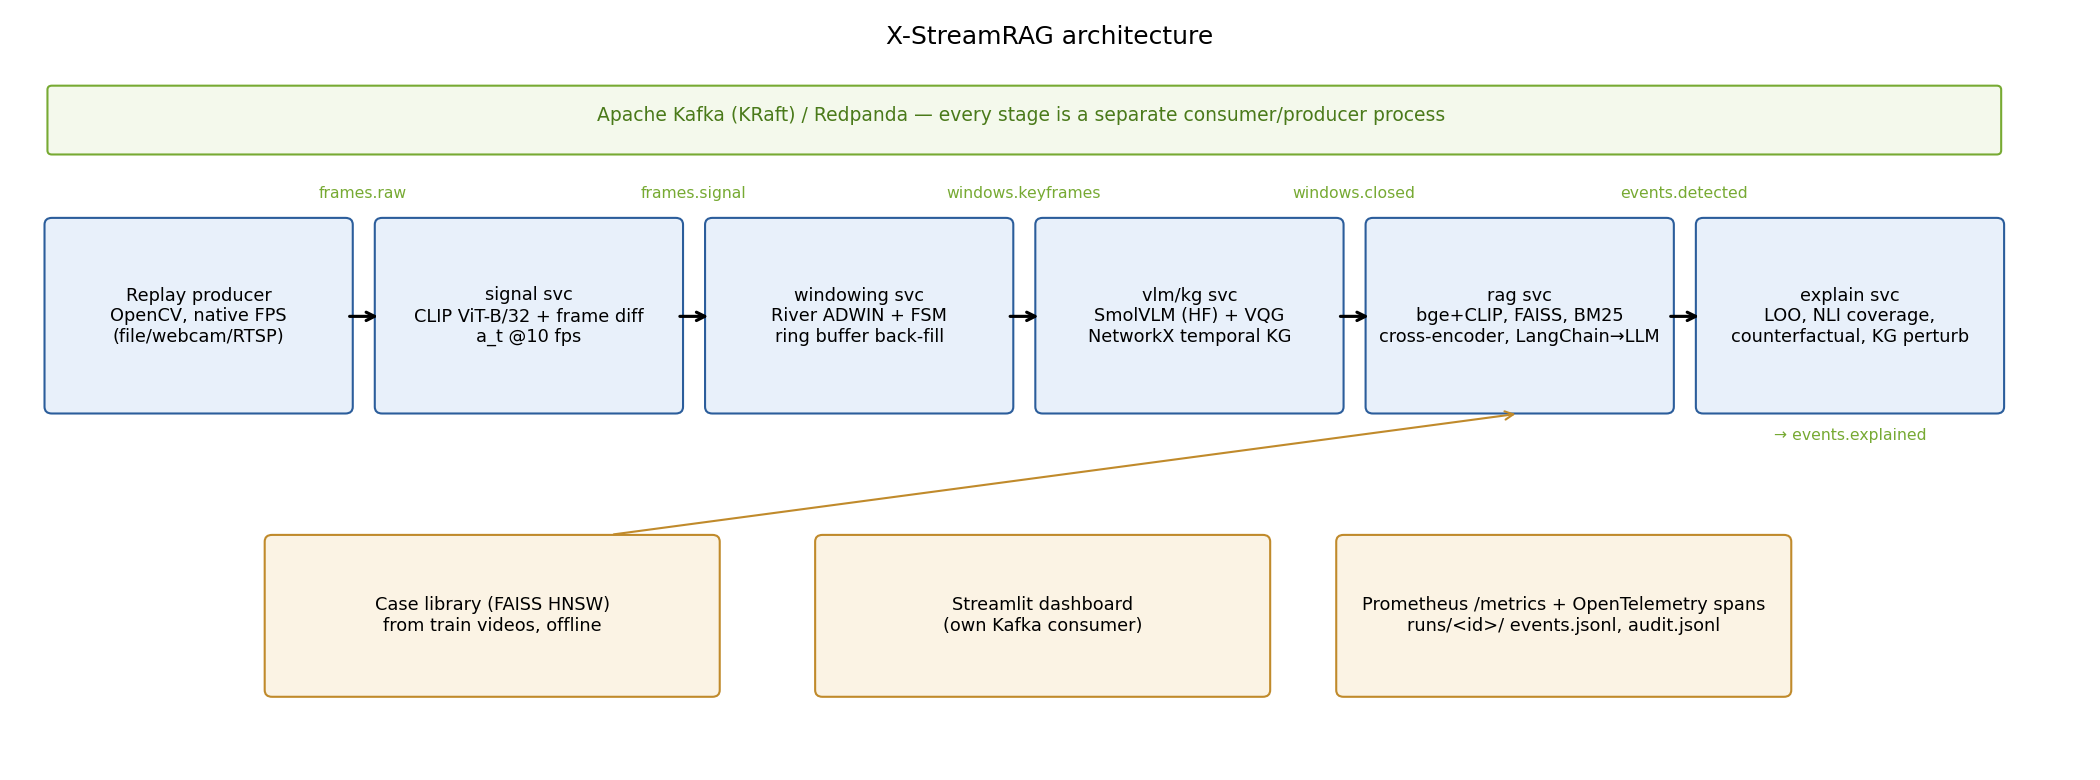
\includegraphics[width=\textwidth]{architecture.png}
\caption{X-StreamRAG architecture. Each box is a separate process; every arrow is a Kafka topic.}
\label{fig:arch}
\end{figure*}

Fig.~\ref{fig:arch} shows the pipeline. A \textbf{replay producer} (OpenCV) reads a video file, webcam or
RTSP source and publishes each frame as a JPEG (640\,px wide) to the topic \texttt{frames.raw}, released at
the source's native frame rate. Messages are keyed by \texttt{source\_id}, and headers carry the frame id,
video timestamp and ingest timestamp. Each downstream stage is an independent consumer/producer process
with its own consumer group:
\texttt{frames.raw}$\rightarrow$\textbf{signal}$\rightarrow$\texttt{frames.signal}$\rightarrow$\textbf{windowing}$\rightarrow$\texttt{windows.keyframes}$\rightarrow$\textbf{VLM/KG}$\rightarrow$\texttt{windows.closed}$\rightarrow$\textbf{RAG}$\rightarrow$\texttt{events.detected}$\rightarrow$\textbf{explain}$\rightarrow$\texttt{events.explained}.
An end-of-stream marker propagates through all topics so that each stage flushes its per-source state.

\textbf{Signal service.} At about 10\,fps it computes
$a_t = 0.6\,(1-\cos(\mathbf{c}_t,\mathbf{c}_{t-1})) + 0.4\,\overline{|g_t-g_{t-1}|}/255$,
where $\mathbf{c}_t$ is the CLIP ViT-B/32 image embedding and $g_t$ a downscaled gray image. The CLIP
embedding is forwarded and reused later for visual retrieval.

\textbf{Windowing service} (Sec.~\ref{sec:enh}). It owns the 3\,s ring buffer and emits closed windows with
their keyframes.

\textbf{VLM/KG service.} SmolVLM-256M-Instruct~\cite{smolvlm} writes one caption per keyframe and answers
up to five questions from a hand-written traffic knowledge base. Yes/no answers are scored as
$P(\text{yes})$ from next-token logits. A rule-based Visual Query Generator, $Q_{t+k}=\mathrm{VQG}(S_t,KB)$,
adds follow-up questions; for example, ``two vehicles touching = yes'' leads to asking whether a person is
lying near the vehicles. Answers become triples in a NetworkX temporal KG with stable IDs (e.g. \texttt{T17}),
and nodes older than 120\,s are pruned. Every VLM call is cached in SQLite.

\textbf{RAG service.} It embeds the window text summary with bge-small-en-v1.5 and fuses it with the mean
CLIP embedding ($s=0.7\cos_{text}+0.3\cos_{clip}$). Candidate evidence comes from a LangChain retriever
over a FAISS HNSW case library and a recency-constrained session memory, plus BM25, the current window's
caption/VQA units (F$*$) and its KG 1-hop triples (T$*$). A cross-encoder (ms-marco-MiniLM-L-6) keeps the
top 8 units. A LangChain prompt$\rightarrow$LLM$\rightarrow$JSON chain (Qwen2.5-1.5B-Instruct) returns
\{event\_type, start/end, sequence, explanation with [IDs]\}. Confidence is never self-reported: we softmax
the log-probabilities of the seven label strings. An event opens when $P(\text{event})\ge0.5$ in 2 of the
last 3 windows and closes after 2 negative windows.

\textbf{Explain service} (Sec.~\ref{sec:enh}). It consumes \texttt{events.detected} off the hot path and
writes one audit record per event.

\textbf{Monitoring.} Every service exposes Prometheus metrics (frames ingested, FPS, per-stage latency
histograms, VLM calls, end-to-end alert latency, window state) scraped every 1\,s, plus OpenTelemetry
spans per window. A Streamlit dashboard with its own Kafka consumer shows the live frame, the state badge,
the $a_t$ timeline, event cards with clickable evidence IDs, and the explainability panels.

% ------------------------------------------------------------------------------------------------
\section{Proposed Enhancement}\label{sec:enh}
\textbf{What is new.} Relative to StreamingRAG, we replace fixed-rate frame-level decisions with
change-point-driven adaptive windows and window-level hybrid retrieval, and we add a measurable
explainability layer. Relative to TD-RAG, windows are adaptive rather than of fixed length, and they are
applied to video. Relative to CityCopilot-X, attribution and counterfactuals operate on multimodal
streaming evidence: frames, VQA answers, KG triples and past windows.

\textbf{Adaptive windows.} ADWIN~\cite{adwin} ($\delta=0.002$) on $a_t$ marks change points that close
windows. A state machine enters ALERT when $a_t>\mu+3\sigma$ over a rolling 30\,s window (with an absolute
minimum rise of 0.02), when ADWIN fires, or when a hazard is fed back from downstream. It returns to CALM
after 10\,s of calm. The states sample 0.5, 2 and 4 keyframes/s with maximum window lengths of 16, 4 and
2\,s. Within each sampling interval the frame with the highest $a_t$ is chosen (priority scheduling).

\textbf{Pre-event back-fill.} On the CALM$\rightarrow$ALERT transition, the two highest-$a_t$ frames of
the last 3\,s are also sent to the VLM, so a 1\,s collision that falls between two CALM samples is still seen.

\textbf{Fair budget.} A token bucket limits B3 to the same average VLM keyframes/min as the fixed-window
variant (60/min), so adaptivity can only redistribute VLM calls, never add more.

\textbf{Sequence context and hybrid retrieval.} The query is the current window plus the previous two, and
dense, BM25 and KG candidates are merged and reranked. Every stage's score is logged per evidence unit.

\textbf{Explainability (E1--E6).}
E1: leave-one-out attribution $w_i=P(y\mid U)-P(y\mid U\setminus\{u_i\})$.
E2: weights projected on the timeline, giving the top-1 timestamped unit for a temporal pointing game.
E3: claim coverage via NLI entailment (DeBERTa-v3-small, $p\ge0.5$) of each explanation sentence against
its cited units, plus token coverage.
E4: counterfactual removal of the top-$k$ vs.\ random-$k$ units ($k\in\{1,2,3\}$, 5 seeds), reporting
$\Delta$confidence, flip rate and the faithfulness gap $\Delta\text{conf}_{top}-\Delta\text{conf}_{rand}$.
E5: KG triple/entity/relation removal.
E6: an embedding-drift monitor over window centroids.

% ------------------------------------------------------------------------------------------------
\section{Implementation}
\textbf{Stream and data.} The public UCF-Crime test videos (our proposal's main test set) could not be
downloaded on the development laptop. We therefore replay 14 traffic clips: 12 accident clips (2 fixed
CCTV, 9 dashcam, 1 news fire) and 2 normal clips, from public GitHub repositories and Intel's CC-BY sample
videos. They total 197.5\,s of video, or 5,396 frames, published to Kafka at native FPS. Two
further normal clips (50\,s and 54\,s) were dropped to meet the deadline. Labels are per video. The case
library (TD-RAG's historical windows) has 84 four-second windows and 309 keyframes from the same 16 clips,
each with its video label. At query time, retrieval excludes the query's own video (leave-one-video-out).

\textbf{Configurations.} \textbf{B1} (StreamingRAG re-implementation): 2\,fps keyframes, each keyframe
its own unit, frame-level kNN over keyframe texts, KG and VQG, no explainability. \textbf{B3}
(X-StreamRAG): adaptive windows with back-fill at 60 keyframes/min, sequence context, hybrid retrieval with
rerank, and E1--E5. Both use the same VLM, LLM, prompt, knowledge base and event logic. Experiments run in
fast-replay mode (timestamps preserved), and LLM feedback to the windowing FSM is disabled for
determinism. The explain stage runs after detection because the 16\,GB laptop cannot hold two copies of the
LLM.

\textbf{Tools and versions.} Apache Kafka 3.9.1 (KRaft, WSL2), confluent-kafka 2.11.1, River 0.22.0,
OpenCV 4.11, PyTorch 2.8 (CPU), transformers 4.56.2, sentence-transformers 5.1.1, FAISS 1.12, rank-bm25
0.2.2, NetworkX 3.6.1, LangChain-core 0.3.76, Streamlit 1.50, Prometheus 2.54.1, OpenTelemetry SDK 1.37,
Python 3.13. Hardware: Intel i5-1340P, 16\,GB RAM, no GPU. Seeds are fixed, and the configuration, git
commit and library versions are saved with every run.

\textbf{Design choice.} Qwen2.5-0.5B was tried first and rejected because it assigned
$P(\text{collision})>0.99$ to a calm highway window. With an explicit ``default to none'' instruction,
Qwen2.5-1.5B gives $P(\text{none})=0.96$ for that window and $P(\text{collision})\approx0.99$ for a crash
window.

% ------------------------------------------------------------------------------------------------
\section{Experimental Setup and Results}
\textbf{Metrics.} Video-level accuracy, precision, recall and F1 (a video is positive if any event is
raised), with 95\% bootstrap CIs over videos (1,000 resamples) and an exact McNemar test between B1 and
B3. We also report the frame-processing ratio, VLM keyframes/min, window close$\rightarrow$verdict latency,
throughput, retrieval P@5, and the E1--E5 explainability metrics. Event-level metrics (tIoU$\ge$0.1 or start
within $\pm$2\,s of the GT segment, short-event recall, detection delay, pointing game) need annotated
event times, which are not yet available for the dev clips, so they are omitted.

\begin{table}[t]
\caption{Main comparison on 14 clips (12 accident, 2 normal). Source: results/summary.csv}
\label{tab:main}
\centering
\begin{tabular}{lcc}
\toprule
Metric & B1 StreamingRAG & B3 X-StreamRAG \\
\midrule
Video accuracy & 0.857 & 0.571 \\
Precision / Recall & 0.857 / 1.000 & 0.875 / 0.583 \\
F1 [95\% CI] & 0.923 [0.78, 1.00] & 0.700 [0.44, 0.88] \\
False alarms (normal clips) & 2 / 2 & 1 / 2 \\
Windows (LLM calls) & 402 & 50 \\
VLM keyframes / min & 122.1 & 83.2 \\
Frame-processing ratio & 0.074 & 0.051 \\
Window latency P50 / P95 (s) & 2476 / 4904 & 1377 / 3851 \\
Retrieval P@5 & 0.581 & 0.888 \\
\bottomrule
\end{tabular}
\end{table}

\begin{table}[t]
\caption{Explainability of B3 events (E1--E5). Source: results/b3-main/metrics.json}
\label{tab:xai}
\centering
\begin{tabular}{lccc}
\toprule
 & $k=1$ & $k=2$ & $k=3$ \\
\midrule
$\Delta$conf, top-$k$ removed & 0.081 & 0.106 & 0.114 \\
$\Delta$conf, random-$k$ removed & 0.020 & 0.040 & 0.091 \\
Faithfulness gap & 0.061 & 0.066 & 0.023 \\
Flip rate top / random & 0.25 / 0.23 & 0.25 / 0.20 & 0.25 / 0.23 \\
\midrule
\multicolumn{4}{l}{Claim coverage 0.00, token coverage 0.00, unsupported 1.00 ($n=8$ events)} \\
\bottomrule
\end{tabular}
\end{table}

\begin{figure}[t]
\centering
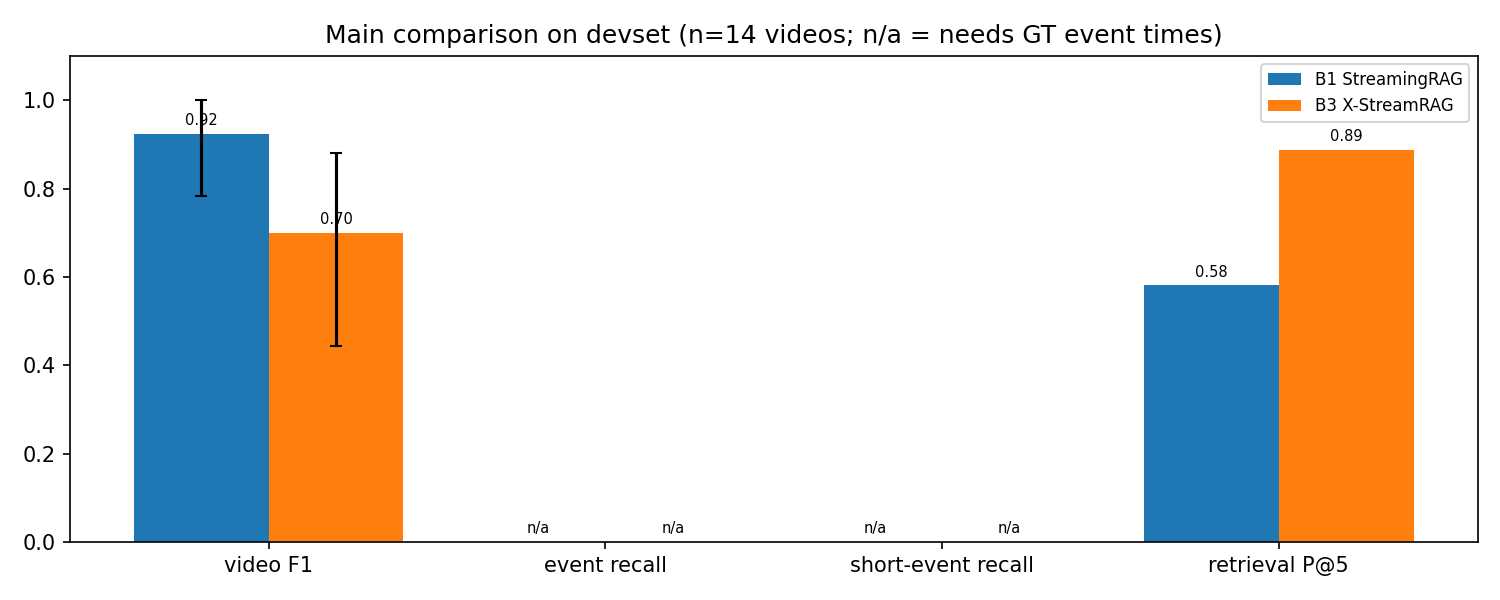
\includegraphics[width=\columnwidth]{main_results.png}
\caption{B1 vs B3 on the 14-clip stream.}
\label{fig:main}
\end{figure}

\begin{figure}[t]
\centering
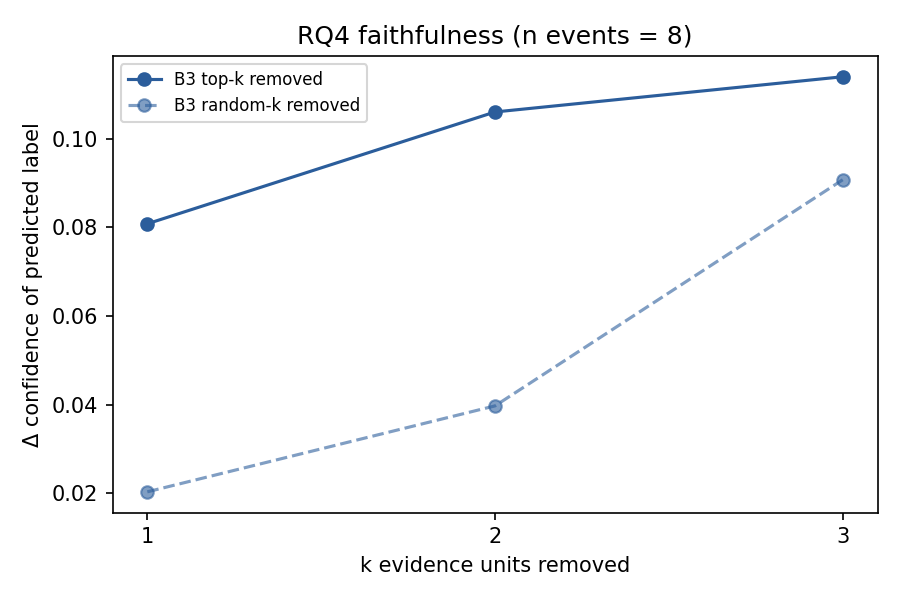
\includegraphics[width=\columnwidth]{faithfulness.png}
\caption{RQ4: confidence drop when the top-$k$ attributed vs.\ random-$k$ evidence units are removed.}
\label{fig:faith}
\end{figure}

\textbf{Detection.} Table~\ref{tab:main} and Fig.~\ref{fig:main} show that the frame-level baseline detects
more accident clips. B1 raised an event on all 12 accident clips (recall 1.00) but also on both normal clips,
so its precision is 0.857. B3 raised events on 7 of 12 accident clips (recall 0.583) and on one normal clip
(precision 0.875). Per video, B1 was right on 5 clips where B3 was wrong and B3 on 1 clip where B1 was wrong;
the exact McNemar test gives $p=0.22$, so with 14 clips neither system is significantly better. Event types
were correct on every detected clip for both systems.

\textbf{Compute and latency.} B3 groups the same 197.5\,s of video into 50 windows instead of 402, i.e.\ 8$\times$
fewer LLM calls, and processes 5.1\% of frames with the VLM against 7.4\% (83 vs.\ 122 keyframes/min).
Its window latency is lower (P50 1377\,s vs.\ 2476\,s) even though each B3 LLM call is longer (P50 98\,s vs.\
13\,s per window), because the window prompt carries sequence context and eight reranked evidence units.
Both latencies are dominated by queueing in fast-replay mode on a CPU (Sec.~\ref{sec:disc}) and are not
real-time. Window-level hybrid retrieval returns more relevant cases: P@5 rises from 0.58 to 0.89.

\textbf{Explainability.} Table~\ref{tab:xai} and Fig.~\ref{fig:faith} cover the 8 B3 events. Removing the
top-1 attributed unit lowers confidence by 0.081, four times the drop from removing a random unit (0.020);
at $k=2$ the ratio is 2.7$\times$. At $k=3$ the gap shrinks to 0.023 because random removals start to hit
important units too. Flip rates barely differ (0.25 top vs.\ 0.20--0.23 random), and the absolute drops are
small because confidence is saturated (0.97--0.997 on every event). Claim coverage is 0: in all 8 events the
LLM wrote a fluent explanation but cited no evidence IDs, so no claim could be checked against its sources.

% ------------------------------------------------------------------------------------------------
\section{Discussion and Inferences}\label{sec:disc}
\textbf{Short clips.} All five accident clips that B3 missed (2.9--6.1\,s long) produced exactly one window:
the change detector stayed in CALM, whose windows may last up to 16\,s, so the whole clip became a single
window. The LLM scored each of these windows correctly ($P(\text{event})=0.90$--$0.92$, type
\texttt{vehicle\_collision}), but the 2-of-3 debounce needs two positive windows, so no event opened. Every
B3 clip with two or more windows was detected. B1 cuts a window every 0.5\,s (6--13 windows on the same
clips) and never meets this limit, so the shared debounce rule penalises only the adaptive method. The rule
should count seconds of positive evidence rather than windows.

\textbf{The LLM is not discriminating.} Every B3 window scored $P(\text{event})\ge0.5$, including those of
both normal clips; \texttt{dashcam\_negative\_samples\_10} was classed correctly only because it was also a
single window. If single positive windows could open an event, B3 would give 12 TP, 2 FP and 0 TN, exactly
B1's result. On this set, therefore, the detection gap between B1 and B3 comes from window counts and the
debounce, not from better or worse evidence, and it says nothing yet about whether adaptive windows help.

\textbf{False alarms.} \texttt{intel\_car-detection}, a 30\,s normal parking-lot clip, was flagged by B3 in all
8 windows (confidence 0.987). The explanation reads ``a collision between vehicles as evidenced by the
presence of multiple vehicles and people'': the LLM equates a busy scene with a collision. Its strongest
attributions are the current window's own captions (F3 0.034, F1 0.033), and every unit weighs under 0.04,
so no single piece of evidence drove the decision. Together with the saturated confidences, this shows the
label-probability confidence is poorly calibrated, and 0.5 is far too low a threshold.

\textbf{Explanations.} A positive faithfulness gap at every $k$ means the attribution ranking is better than
chance at finding the evidence the model relies on, so E1 is informative. The effect is small, however, and
the flip rates are close to random. The larger problem is grounding: the 1.5B LLM ignored the instruction to
cite evidence IDs in all 8 events, so the explanations cannot be audited claim by claim (claim coverage 0).
The pipeline measures this failure instead of hiding it, which is the purpose of the explainability layer.

\textbf{Threats to validity.} The test set is small (14 clips) and mostly dashcam, while the target is fixed
CCTV. The case library comes from the same pool as the test set (leave-one-video-out), which may inflate
retrieval quality. Event times are not annotated, so short-event recall (RQ3) and the pointing game (RQ2)
are not measured. The fixed-window variant (B2) was not run, so the effect of adaptivity cannot be separated
from that of windowing and hybrid retrieval. B3's measured VLM rate (83 keyframes/min) is above the
60/min target of the token bucket, so the budget match is approximate. Everything runs on a CPU, so latency
is far from real time (P50 11.7--14.1\,s per VLM keyframe; 12.7\,s per B1 and 98.5\,s per B3 LLM window;
real-time factor 0.05), and the throughput numbers reflect this laptop, not the method.

% ------------------------------------------------------------------------------------------------
\section{Conclusion and Future Work}
We built X-StreamRAG, a Kafka-based streaming RAG pipeline that reproduces StreamingRAG as a baseline and
extends it with adaptive temporal windows, window-level hybrid retrieval and a measurable explainability
layer. On 14 clips it matched the baseline's precision with 8$\times$ fewer LLM calls and much better retrieval,
but missed five short clips because of a window-count debounce, and its explanations were faithful only
weakly and cited no evidence. Future work: calibrating the event threshold, evaluation on UCF-Crime and TAD with annotated event
times, the fixed-window and budget-sweep experiments for RQ3, a window-length-aware debounce, GPU
deployment for real-time latency, and a human rating of explanation quality.

\begin{thebibliography}{00}
\bibitem{streamingrag} M. Sankaradas, R. K. Rajendran, and S. T. Chakradhar, ``StreamingRAG: Real-time contextual retrieval and generation framework,'' in \emph{Proc. AI4Sys}, 2024, arXiv:2501.14101.
\bibitem{tdrag} \Xu, Deng, and Jin, ``TD-RAG: Time-aware dynamic-window RAG for risk early warning,'' in \emph{Proc. IEEE CyberSciTech}, 2025.
\bibitem{citycopilot} \Gudipati \emph{et al.}, ``CityCopilot-X: A real-time explainability panel for RAG,'' in \emph{Proc. IEEE ICAIC}, 2026, doi:10.1109/ICAIC67076.2026.
\bibitem{adwin} A. Bifet and R. Gavald\`a, ``Learning from time-changing data with adaptive windowing,'' in \emph{Proc. SIAM SDM}, 2007.
\bibitem{clip} A. Radford \emph{et al.}, ``Learning transferable visual models from natural language supervision,'' in \emph{Proc. ICML}, 2021.
\bibitem{smolvlm} A. Marafioti \emph{et al.}, ``SmolVLM: Redefining small and efficient multimodal models,'' arXiv:2504.05299, 2025.
\bibitem{faiss} M. Douze \emph{et al.}, ``The FAISS library,'' arXiv:2401.08281, 2024.
\bibitem{bm25} S. Robertson and H. Zaragoza, ``The probabilistic relevance framework: BM25 and beyond,'' \emph{Found. Trends Inf. Retr.}, vol. 3, no. 4, 2009.
\bibitem{rag} P. Lewis \emph{et al.}, ``Retrieval-augmented generation for knowledge-intensive NLP tasks,'' in \emph{Proc. NeurIPS}, 2020.
\bibitem{contextcite} B. Cohen-Wang \emph{et al.}, ``ContextCite: Attributing model generation to context,'' in \emph{Proc. NeurIPS}, 2024.
\bibitem{ucf} W. Sultani, C. Chen, and M. Shah, ``Real-world anomaly detection in surveillance videos,'' in \emph{Proc. CVPR}, 2018.
\bibitem{streamrag2026} \Xie \emph{et al.}, ``StreamRAG: Enhancing real-time video understanding with retrieval augmentation,'' in \emph{Proc. CVPR}, 2026.
\end{thebibliography}

\end{document}
